% This is samplepaper.tex, a sample chapter demonstrating the
% LLNCS macro package for Springer Computer Science proceedings;
% Version 2.20 of 2017/10/04
%
\let\accentvec\vec
\documentclass[runningheads]{llncs}
\let\spvec\vec
\let\vec\accentvec
%
\usepackage{graphicx,amsmath,amssymb,subfigure,url,epsfig,bm}
\usepackage[ruled,boxed]{algorithm2e}
\usepackage[misc]{ifsym}
% \usepackage{spconf,amsmath,epsfig}
% \usepackage{bm,graphicx,subfigure,diagbox,amssymb,amsfonts,url,amsmath,amssymb,amsthm,bm}

% Used for displaying a sample figure. If possible, figure files should
% be included in EPS format.
%
% If you use the hyperref package, please uncomment the following line
% to display URLs in blue roman font according to Springer's eBook style:
% \renewcommand\UrlFont{\color{blue}\rmfamily}

\begin{document}
%
\title{Accelerating Topic Detection on Web for a Large-Scale Data Set via Stochastic Poisson Deconvolution}
%
\titlerunning{Accelerating Topic Detection on Web for a Large-Scale Data Set via SPD}
% If the paper title is too long for the running head, you can set
% an abbreviated paper title here
%
\author{Jinzhong Lin\inst{1} \and
Junbiao Pang\inst{2} \and
Li Su\inst{1} \and
Yugui Liu\inst{1} \and
Qingming Huang\inst{1,3}\textsuperscript{(\Letter)}}
%%
\authorrunning{J. Lin et al.}
%% First names are abbreviated in the running head.
%% If there are more than two authors, 'et al.' is used.
%%
\institute{School of Computer and Control Engineering, University of Chinese Academy of Sciences, Beijing, China \\
\email{lin\_jin\_zhong@outlook.com, \{suli,liuyg,qmhuang\}@ucas.ac.cn} \and
Faculty of Information Technology, Beijing University of Technology, Beijing, China\\
\email{junbiao\_pang@bjut.edu.cn} \and
Institute of Computing Technology, Chinese Academy of Sciences, Beijing, China
% Key Lab on Big Data Mining and Knowledge Management, Chinese Academy of Sciences, Beijing, China
}
%
\maketitle              % typeset the header of the contribution
%
\begin{abstract}
Organizing webpages into hot topics is one of the key steps to understand the trends from multi-modal web data. To handle this pressing problem, Poisson Deconvolution (PD), a state-of-the-art method, recently is proposed to rank the interestingness of web topics on a similarity graph. Nevertheless, in terms of scalability, PD optimized by expectation-maximization is not sufficiently efficient for a large-scale data set. In this paper, we develop a Stochastic Poisson Deconvolution (SPD) to deal with the large-scale web data sets. Experiments demonstrate the efficacy of the proposed approach in comparison with the state-of-the-art methods on two public data sets and one large-scale synthetic data set.

\keywords{Large-scale \and Poisson Deconvolution \and Unsupervised Ranking \and Web Topic Detection \and Surrogate Function.}
\end{abstract}
%
%
%
\section{Introduction}
\label{sec:intro}
With the rapid development of information technology and mobile internet, social media websites greatly facilitate both the generation and the propagation of User-Generated Content (UGC). Consequently, the unprecedented explosion in the volume of UGC~\cite{pang-2013-unsupervised} data makes people difficult to quickly grasp ``hot'' contents. Driven by this practical requirement, topic detection from web~\cite{pang-2013-unsupervised,zhang-2013-cross,pang-tao-2016-lpd} is such an effort to organize webpages into meaningful topics automatically. Different from the traditional Topic Detection and Tracking (TDT)~\cite{allan-1998-TDT} that aims at discovering topics from professionally edited news articles, web topic detection faces a large-scale UGC data which never evolve into any hot topics.
In this paper, web topic detection is formally defined as the task of discovering of a tiny fraction of webpages strongly connected by a seminal hot event from a large amount of social media~\cite{pang-2013-unsupervised}.

The state-of-the-art approach for web topic detection is to rank the interestingness of topics on a similarity graph~\cite{pang-2013-unsupervised,pang-tao-2018-neurocomputing}. Concretely, PD allocates an weight to each topic by diffusing the similarities between webpages~\cite{pang-2013-unsupervised}. Although a similarity graph is not only efficiently constructed by online $k$-Nearest Neighborhood Graph ($k$-N$^2$G)~\cite{debatty-2016-fastonlineknn} but also is efficiently stored as a sparse matrix, one pressing problem is that PD is not efficiently scalable for a large-scale data set. The reason is that PD has to reconstruct a $N\times N$ float matrix at each iteration where $N$ is the number of webpages.

It is natural to ask: \emph{can we exploit a small fraction of data at each iteration for PD?} One of the simple and yet efficient approaches is stochastic optimization~\cite{hannah-2015-Stochastic}. There are at least two potential benefits of this approach: reducing the requirement of the physical memory, and avoiding the reconstruction of a $N\times N$ scale similarity graph. However, PD optimized by EM algorithm has to maintain a hidden variable which has the same scale of the similarity graph.

In this paper, we propose a Stochastic Poisson Deconvolution (SPD) approach to handle a large-scale data set for web topic detection. It iteratively builds a surrogate of the expected objective function when only a small fraction of data are observed at each iteration. Meanwhile, only a few small stochastically sampled data are used to update the surrogate function. Therefore, avoiding loading all data into memory, SPD significantly reduces the running time.

To the best of our knowledge, this is the first to handle the scalability of PD for web topic detection. The proposed method is conceptually simple and yet efficiently. On a large-scale data set, SPD leads to drastic training-time improvement, \emph{e.g.}, approximate 12.6$\times$ speedup on a toy data set with about 200,000 webpages. Meanwhile, SPD can achieve the similar performances to that of PD on two public data sets.

The rest of this paper is organized as follows: Section~\ref{sec:relatedwork} reviews the related work. We describe the details of our approach in Section~\ref{sec:coupledframework}. Experimental results are presented in Section~\ref{sec:results}, and the paper is concluded in Section~\ref{sec:conclusion}.
%
%
%
\section{Related Work}
\label{sec:relatedwork}
\textbf{Detect Web Topic from Multi-modal Data.} Recognizing that webpages are the typical heterogeneous data, many literatures consider web topic detection as the clustering task from the multi-modal data. There are two important research threads. One is the multi-modal-based method~\cite{blei-lafferty-2007-correlatedtopicmodel,putthividhy-2010-multimodalLDA}, and the other is the similarity graph-based method~\cite{papadopoulos-2011-cluster}.

In the former thread, topic detection extends the single-modality based approaches into multi-modal data. For instance, multi-modal LDA~\cite{putthividhy-2010-multimodalLDA}, a variation of LDA~\cite{blei-2003-LDA}, is proposed to detect topics from both the images and their tags. In the similarity graph-based method, multi-modal information is fused into the edges of a graph, where the vertexes are clustered into different topics. For instance, Wu \emph{et al.}~\cite{wu-2007-crosslingual} detect topics of news videos by fusing the similarities from Nearly-Duplicated Keyframes (NDKs) and the speech transcripts.

Compared with the multi-modal-based topic modelings~\cite{putthividhy-2010-multimodalLDA}, similarity graph-based approach is easily extendable for the other algorithms~\cite{aiello-2013-sensing,papadopoulos-2011-cluster,cao-2011-tracking}. SPD belongs to the similarity graph-based approach. However, our method does not aim at improving accuracy of the detection system, but rather making PD scalable for a large scale data set.

Despite many approaches propose to detect topics in social media, to the best of our knowledge, only a few solutions try to parallelize LDA, \emph{e.g.},~\cite{wang-2009-PLDA,chen-2015-WarpLDA,Liu-2011-PLDA+}. As discussed in~\cite{pang-2013-unsupervised,pang-tao-2016-lpd}, LDA assumes that each webpage should belong to a topic. In fact, in terms of web topic detection, almost 90\% webpages would not evolve into any hot topics. Therefore, the paralleled LDAs are incapable to remove the low-valued webpages which do not develop into hot topics.

\textbf{Stochastic Optimization.} Stochastic optimization refers to the minimization (or maximization) of a function in the presence of randomness. The randomness may be presented as noises in measurements, Monte Carlo randomness during the search, or both~\cite{hannah-2015-Stochastic}. For instance, Stochastic Gradient Descent (SGD) and its variants~\cite{mairal-2013-optimization,johnson-2013-sgd-accelerating,Roux-2012-sgd-exponential} has been popular in machine learning due to their efficiency and effectiveness. However, the objective function of PD is iteratively changed at each expectation step. This makes SGD unusable for the EM-based PD.

Majorization-Minimization (MM)~\cite{lange-2000-optimization}, a generalization of EM~\cite{cappe-2009-online-EM,neal-1998-view-EM}, iteratively minimizes a surrogate function that is the upper bound of the objective function. Many approaches can be interpreted as MM, such as variational Bayes~\cite{Wainwright-2008-variational-bayes} and proximal algorithms~\cite{beck-2009-fastshrinkage}. Recently, Stochastic MM (SMM)~\cite{mairal-2013-SMM} is proposed to make MM scalable.

Inspired by the success of warm restart and SMM~\cite{mairal-2013-SMM}, our proposed method additively updates a surrogate function. The resulting SPD not only stores a few random sampled edges, but also significantly speeds up the convergence speed in practice. To the best of our knowledge, this paper is first to apply the surrogated-based method to accelerate PD for web topic detection.
%
%
\section{Stochastic Poisson Deconvolution}
\label{sec:coupledframework}
\subsection{Revisit Poisson Deconvolution}
Given a set of webpages $\mathcal{X}=\{\mathbf{x}_1,\ldots,\mathbf{x}_N\}$, we convert these webpages into a similarity graph $G=(V,E,A)$, where the vertex set $V$ corresponds to the webpages $\mathcal{X}$, the elements of affinity matrix $A$ $(a_{ij}\in A)$ corresponds to the scaled and truncated similarities between webpages $\mathcal{X}$, and the edge set $E$ ($e_{ij}\in E$) corresponds to the similarities between webpages $\mathcal{X}$. The details about how to build a similarity graph can be founded in~\cite{pang-tao-2016-lpd}.

A set of multi-granularity topics $C_k$ ($k=1,\ldots,K$) are generated from a similarity graph $G$, where a topic $C_k$ is represented as:
\begin{equation}\label{eqt:ck}
C_{k} = c^{\top}_k{\circ} c_k,
\end{equation}
in which the indicator vector $ c_k \in \{0, 1\}^{1\times N}$, where $1$ or $0$ means that whether the topic $C_k$ contains the webpage $\mathbf{x}_i$ or not. The operation $\circ$ means that the diagonal of the matrix $c^{\top}_k c_k$ is set to be zero.

Given a set of topics $\{C_1,\ldots, C_K\}$ and a similarity Graph \mbox{$G=(V,E,A)$}, the topic-wise weight $\mu_k$ of a topic $C_k$ is learned under Poisson noise as follows:
\begin{equation} \label{eqt:poissondeconvolution}
\begin{split}
w_{ij} & \sim \text{Poisson}(a_{ij})\\
where & \ \ w_{ij} = \sum_{k=1}^{K} \mu_k C_{k_{ij}}.
\end{split}
\end{equation}
The interestingness of a topic is estimated as $i_k=\mu_k\cdot |C_k|$, where $|C_k|$ is the number of webpages in the topic $C_k$.

By applying EM algorithm, PD~\eqref{eqt:poissondeconvolution} is iteratively solved as follows:
\begin{equation} \label{eqt:iterationofPD}
    \mu_k = \frac{\sum_{a_{ij}\in C_k} a_{ij} P_{k_{ij}}}{\sum_{a_{ij}\in C_k} C_{k_{ij}}},
\end{equation}
where $P_{k_{ij}}$ ($\sum_{k=1}^{K} P_{k_{ij}}=1$) are the hidden variables, \empty{i.e.}, $P_{k_{ij}} = \frac{\mu_k C_{k_{ij}}}{\sum_{m=1}^{K}\mu_m C_{m_{ij}}}$~\cite{pang-2013-unsupervised}.

\subsubsection{The Drawback of Poisson Deconvolution:}
Eqt.~\eqref{eqt:iterationofPD} needs to reconstruct all edges in a similarity graph $G$ at each iteration. In practice, a float $N\times N$ matrix has to be allocated in memory; besides, at each iteration, each element of the $N\times N$ matrix has to be updated. Therefore, the time complexity of PD is $O(TN^2)$ where $T$ is the number of iterations; meanwhile, the space complexity of $PD$ is $O(N^2)$. The polynomial complexity handicaps the scalability of PD for a large-scale data set. This problem looms as long as the computation-intensive $N\times N$ matrix is required to be allocated and reconstructed.

\subsection{Stochastic Poisson Deconvolution}
\begin{algorithm}
\small
{
    \SetAlgoLined
    \caption{Stochastic Poisson Deconvolution}
    \label{alg:SMM}
    \KwIn{$G$ (Similarity Graph), $C_k$ $k=1,\ldots,K$ (Topics), $b$ (Batch size), $T$ (Number of iteration);}
    \textbf{Initialization}: cumulative intermediates:$\bar{B}^0=\bar{D}^0=0^{K\rm x 1}$; $W=0^{K\rm x 1}$; $\beta$, $\alpha$; $\bm{\mu}^0$;\\
    \For{$t = 1,\ldots,T$} {
        Randomly draw a few rows of G: $\bar{A}^t$;\\
  %      compute the topic $C_k$ by~\eqref{eqt:ck};\\
        compute the weight by~\eqref{eqt:weightupdate};\\
        compute the temporary variable $B^t_k$, $D^t_k$ by~\eqref{eqt:computebnkanddnk};\\
        update the cumulative intermediates:
            \begin{center}$\bar{B}^t_k = (1-w^t_k)\bar{B}^{t-1}_k + w^t_kB^t_k$;\end{center}
            \begin{center}$\bar{D}^t_k = (1-w^t_k)\bar{D}^{t-1}_k + w^t_kD^t_k$;\end{center}
        update the current estimate: $\mu^t_k = \frac{\bar{B}^t_k}{\bar{D}^t_k};$
    }
    \KwOut{$\bm{\mu}$;}
}
\end{algorithm}

We present SPD for a large-scale data set in Algorithm~\ref{alg:SMM}. At each iteration, by assuming that the edges in a similarity graph are \emph{i.i.d.} from an unknown distribution, we draw a mini-batch edges $\bar{A}^t$ from a similarity graph at the $t$-th iteration. However, in practice, the mini-batch edges are computed by cycling on a randomly permuted training set~\cite{bottou-2007-tradeoffs}, since it is often difficult to obtain true \emph{i.i.d.} samples.

Concretely, the objective function of PD~\eqref{eqt:poissondeconvolution} is equal to the following problem:
\begin{align} \label{eq:objectivefunction}
    &\quad\max{\ln \prod_{a_{ij} \in \bar{A}^t}\text{Poisson}(a_{ij})}  \notag\\
 %   &=\max{\sum_{a_{ij} \in A^t}\ln{\frac{e^{-\sum_{k=1}^{K} \mu_k C_{k_{ij}}} (\sum_{k=1}^{K}\mu_k C_{k_{ij}})^{a_{ij}}}{a_{ij}!}}}\notag\\
  &\Leftrightarrow\min \underbrace{\frac{1}{b}{\sum_{a_{ij} \in \bar{A}^t} \Big(\sum_{k=1}^{K}\mu_k C_{k_{ij}} - a_{ij}\ln \sum_{k=1}^{K}\mu_k C_{k_{ij}}\Big)}}_{f^t(\bar{A}^t,\bm{\mu})},
\end{align}
where $b$ is the number of rows in a mini-batch $\bar{A}^t(\bar{A}^t\in \mathbb{R}^{b \rm x N})$.

Using Jensen's inequality, the upper bound of likelihood function in~\eqref{eq:objectivefunction} is used as the surrogate function:
\begin{align}
    f^t(\bar{A}^t,\bm{\mu}) &\leqslant{\underbrace{\frac{1}{b}\sum_{a_{ij} \in \bar{A}^t} \left(\sum_{k=1}^{K}\mu_k C^t_{k_{ij}} - a_{ij}\sum_{k=1}^{K} P^t_{k_{ij}} \ln \frac{\mu_k C^t_{k_{ij}}}{P^t_{k_{ij}}}\right)}_{J^t(f^t,\bm{\mu}^{t-1})}}.
\end{align}
Where $C^t_{k_{ij}}$ means the $k$-th topic contracted by sampled webpages, $P^t_{k_{ij}}$($\sum_{k=1}^{K}P^t_{k_{ij}}=1)$ is the hidden variable for the $t$-th iteration, \emph{i.e.}, $P^t_{k_{ij}} = \frac{\mu^{t-1}_k C^t_{k_{ij}}}{\sum_{k=1}^{K}\mu^{t-1}_k C^t_{k_{ij}}}$.

The gradient of $J^t(f^t,\mu^{t-1})$ with respect to $\mu_k$ is as follows:
\begin{equation} \label{eqt:computebnkanddnk}
    \frac{d}{d\mu_k}J^t(f^t,\bm{\mu}^{t-1})=\underbrace{\frac{1}{b}\sum_{a_{ij}\in \bar{A}^t}C^t_{k_{ij}}}_{D^t_k} - \underbrace{\frac{\frac{1}{b}\sum_{a_{ij}\in \bar{A}^t} a_{ij}P^t_{k_{ij}}}{\mu_k}}_{B^t_k},
\end{equation}
where $D^t_k\in \mathbb{R}^{1 \rm x 1}$ and $B^t_k\in \mathbb{R}^{1 \rm x 1}$ are the temporal variables.

\newtheorem{mydef}{Definition}
\newtheorem{mythe}{Theorem}
\newtheorem{mypro}{Proposition}
\newtheorem{mylemma}{Lemma}

\begin{mypro}(Iterative Update Process) Given the temporal variables $B^t_k$ and $D^t_k$, $\mu_k$ can be iteratively updated as follows:
\begin{equation} \label{eqt:updatemu}
    \mu^t_k = \frac{\bar{B}^t_k}{\bar{D}^t_k}, \quad s.t.:\quad k \in \{k|\exists C^t_{k_{ij}} \neq 0\}
\end{equation}
where
\begin{equation} \label{eqt:iterativeupdating}
\begin{split}
    \bar{B}^t_k \leftarrow (1-w^t_k)\bar{B}^{t-1}_k + w^t_kB^t_k,\\
    \bar{D}^t_k \leftarrow (1-w^t_k)\bar{D}^{t-1}_k + w^t_kD^t_k,
\end{split}
\end{equation}
where the weight $w^t_k$ for the $t$-th iteration is as follows:
\begin{equation} \label{eqt:weightupdate}
    w^t_k = \beta\sqrt{\frac{1+\alpha}{W_k+\alpha}},
\end{equation}
in which $  W_k = W_k + 1, \quad \beta \in (0,1], \qquad \alpha \geq 0$.
\end{mypro}

\begin{proof}
Following the suggestions in SMM~\cite{mairal-2013-SMM}, the combination of the approximate surrogate and the current estimation is as follows :
\begin{equation} \label{eqt:exponentiallyweightedmovingaverage}
    \bar{J}^t_k \leftarrow (1-w^t_k)\bar{J}^{t-1}_k + w^t_k J^t_k,
\end{equation}
$\mu_k$ is optimized by minimizing~\eqref{eqt:exponentiallyweightedmovingaverage}, \emph{i.e.},  $\mu^t_k = \arg \min \bar{J}^t_k(\mu)$. This process can be derived like following:

When $t=m$, solving for $\mu^m_k$ in~\eqref{eqt:exponentiallyweightedmovingaverage} by~\eqref{eqt:computebnkanddnk}~\eqref{eqt:updatemu}~\eqref{eqt:iterativeupdating} can get
\begin{equation}
\mu^m_k = \frac{(1-w^m_k)\bar{B}^{m-1}_k+w^m_kB^m_k}{(1-w^m_k)\bar{D}^{m-1}_k+w^m_kD^m_k} = \frac{\bar{B}^m_k}{\bar{D}^m_k}.
\end{equation}
Finally, without loss of generality, we can get $\mu^t_k$ in the iterative update process~\eqref{eqt:updatemu}~\eqref{eqt:iterativeupdating}.
\end{proof}
The weight $w$ plays a role of Exponentially Weighted Moving Average (EWMA) in approximate surrogate~\eqref{eqt:exponentiallyweightedmovingaverage}. The EWMA is a type
of infinite impulse response filter that represents the exponentially decreased weighting factor. Note that the weight of each older surrogate decreases exponentially but never reaches to zero. The $w$ reflects the importance of the current surrogate; meanwhile $1-w$ reflects the importance of the previous surrogates. Consequently, the older the surrogate is, the smaller the weight should be.
%
%
\section{Experiments and Discusses}
\label{sec:results}
\subsection{Data Sets, Features and Evaluation Criteria}
\textbf{Datasets:} In the experiments, we evaluate our method on two public data sets, \emph{i.e.}, \emph{MCG-WEBV}~\cite{cao-2011-tracking} and \emph{YKS}~\cite{zhang-2013-cross}. MCG-WEBV is first proposed to detect web video topics from the video sharing websites, being downloaded from the ``Most viewed'' videos of ``This month'' on \emph{YouTube}. This data set contains video clips and their titles, tags and descriptions on \emph{Youtube} from Dec. 2008 to Feb. 2009. YKS is a cross-media and cross-platform data set crawled from \emph{YouKu} and \emph{Sina}, respectively. The meta data of YKS contains news articles on \emph{Sina} and titles, tags and descriptions web videos on \emph{YouKu} from May 2012 to June 2012. The statistics of data sets are summarized in Table~\ref{tab:dataset}.

\begin{table}[t!]
\begin{center}
\caption{Summary of data sets in the experiments} \label{tab:dataset}
\begin{tabular}{|c|c|c|c|c|}
  \hline
  Data sets & \#Webpage & \#Topics & $k$ & Sparsity(\%)\\
  \hline\hline
  MCG-WEBV & 3660 & 4240 & 100 & 2.73\\
  \hline
  YKS & 7332 & 5252 & 20 & 0.273\\
  \hline
\end{tabular}
\end{center}
\end{table}

\textbf{Features:} During the pre-processing, MCG-WEBV and YKS are tokenized by \emph{NLTK}\footnote{www.nltk.org} package.
We simply use TF-IDF to encode the textual features. That is, the surrounding text of each video is considered as a set of words. The cosine distance is used to measure the similarity.

\textbf{Evaluation Criteria:}  There are two evaluation methods, \emph{i.e.}, top-10 $F_1$ versus Number of Detected Topics (NDT)~\cite{cao-2011-tracking} and Accuracy versus False Positive Per Topic (FPPT)~\cite{pang-2013-unsupervised}. Note that if two methods have the same top-10 $F_1$ or accuracy score, the one with smaller NDT or FPPT has better performance.

\begin{itemize}
\item \textbf{Top-10 $F_1$ versus NDT:} A detected topic is matched with the ground truth, and then the top 10 $F_1$ scores are averaged to measure the performance of a system:
\begin{eqnarray}
F_1=\frac{2\times Precision \times Recall}{Precision+Recall},
\end{eqnarray}
where $Precision$ is $\frac{|DT \cap GT|}{|DT|}$, $Recall$ is $\frac{|DT \cap GT|}{|GT|}$,
in which $DT$ is a detected topic, $GT$ is a ground truth topic, and $|\cdot |$ denotes the number of webpages in a topic.
\item \textbf{Accuracy versus FPPT:} if a topic is correctly detected, FPPT is the number of false positive topics caused by a detection system. In this paper, accuracy is defined as follows:
\begin{equation}\label{equa:accuracy}
\text{Accuracy}=\frac{\# \text{Successful} }{\# \text{Groundtruth}},
\end{equation}
where $Successful$ means a detected topic $DT$ is successfully discovered, if Normalized Intersected Ratio (NIR) $\frac{|DT \cap GT|}{|DT \cup GT|}$ is larger than a threshold. Following the previous work~\cite{pang-2013-unsupervised}, 0.5 is used as the threshold of NIR in our experiments.
\end{itemize}

For the time efficiency, the curve about the objective function versus the used time is used. More specially, the one with less time to reach convergence has better performance.

\textbf{Enviroment Setting:} To fairly compare our algorithm to the state-of-the-art method, we follow the same setting (\emph{i.e.}, similarity graph and topics) to demonstrate the efficiency of our approach. All experiments are implemented in python with a 3.6 GHz processer and 32G RAM.

\begin{figure}[t!]
\centering
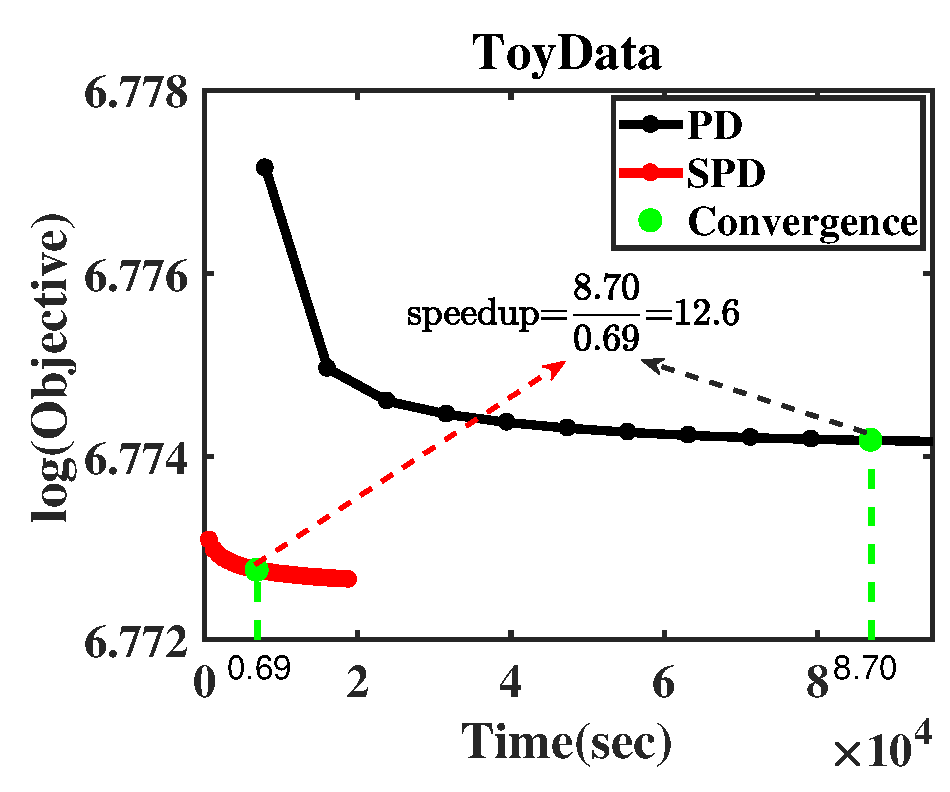
\includegraphics[width=0.5\textwidth]{./results/cmp-objective-toydata/Objective.eps}
\caption{Comparison between PD and SPD on ToyData (best viewed in color).}
\label{fig:toydatacmp}
\end{figure}

\subsection{Analysis of Time Complexity and Space Complexity}
% \subsubsection{Space Complexity}
For PD, a float $N\times N$ matrix has to be allocated in memory to store the reconstructed similarity graph. Therefore, the space complexity and time complexity of PD is $O(N^2)$ and $O(TN^2)$, respectively. In contrast, SPD only updates a small fraction of the reconstructed similarity graph at each iteration. Therefore, SPD only maintains a float $b\times N$ matrix in memory, where $b\times N$ means the size of mini-batch edges (\emph{i.e.}, $\bar{A}^t\in \mathbb{R}^{b \rm x N}$). The space complexity of SPD is $O(bN)$ $(b\ll N)$.
% \subsubsection{Time Complexity}
% PD need to update the float $N\times N$ matrix, leading to a time complexity of $O(TN^2)$ where T is the number of iterations.

\begin{figure}[t!]
\centering
\begin{minipage}{\textwidth}
\subfigure[Objective v.s. Time]
{
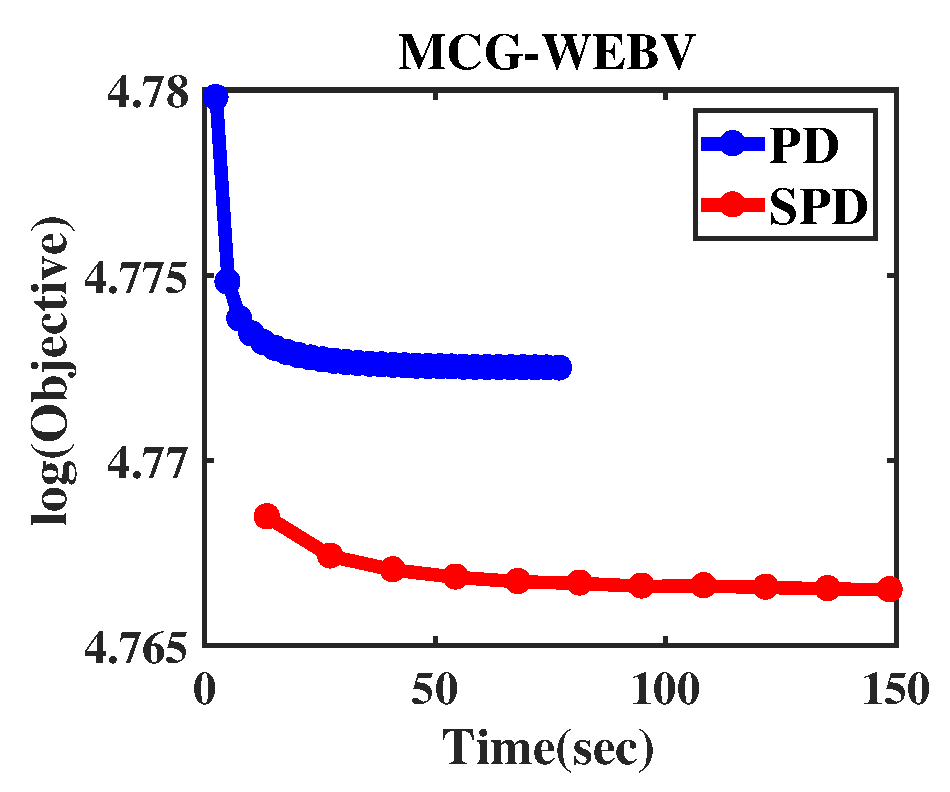
\includegraphics[width=0.31\textwidth,height=.28\textwidth]{./results/cmp-objective-mcg/Objective.eps}
\label{fig:objectivecmponmcg}
}
\subfigure[Accuracy v.s. FPPT]
{
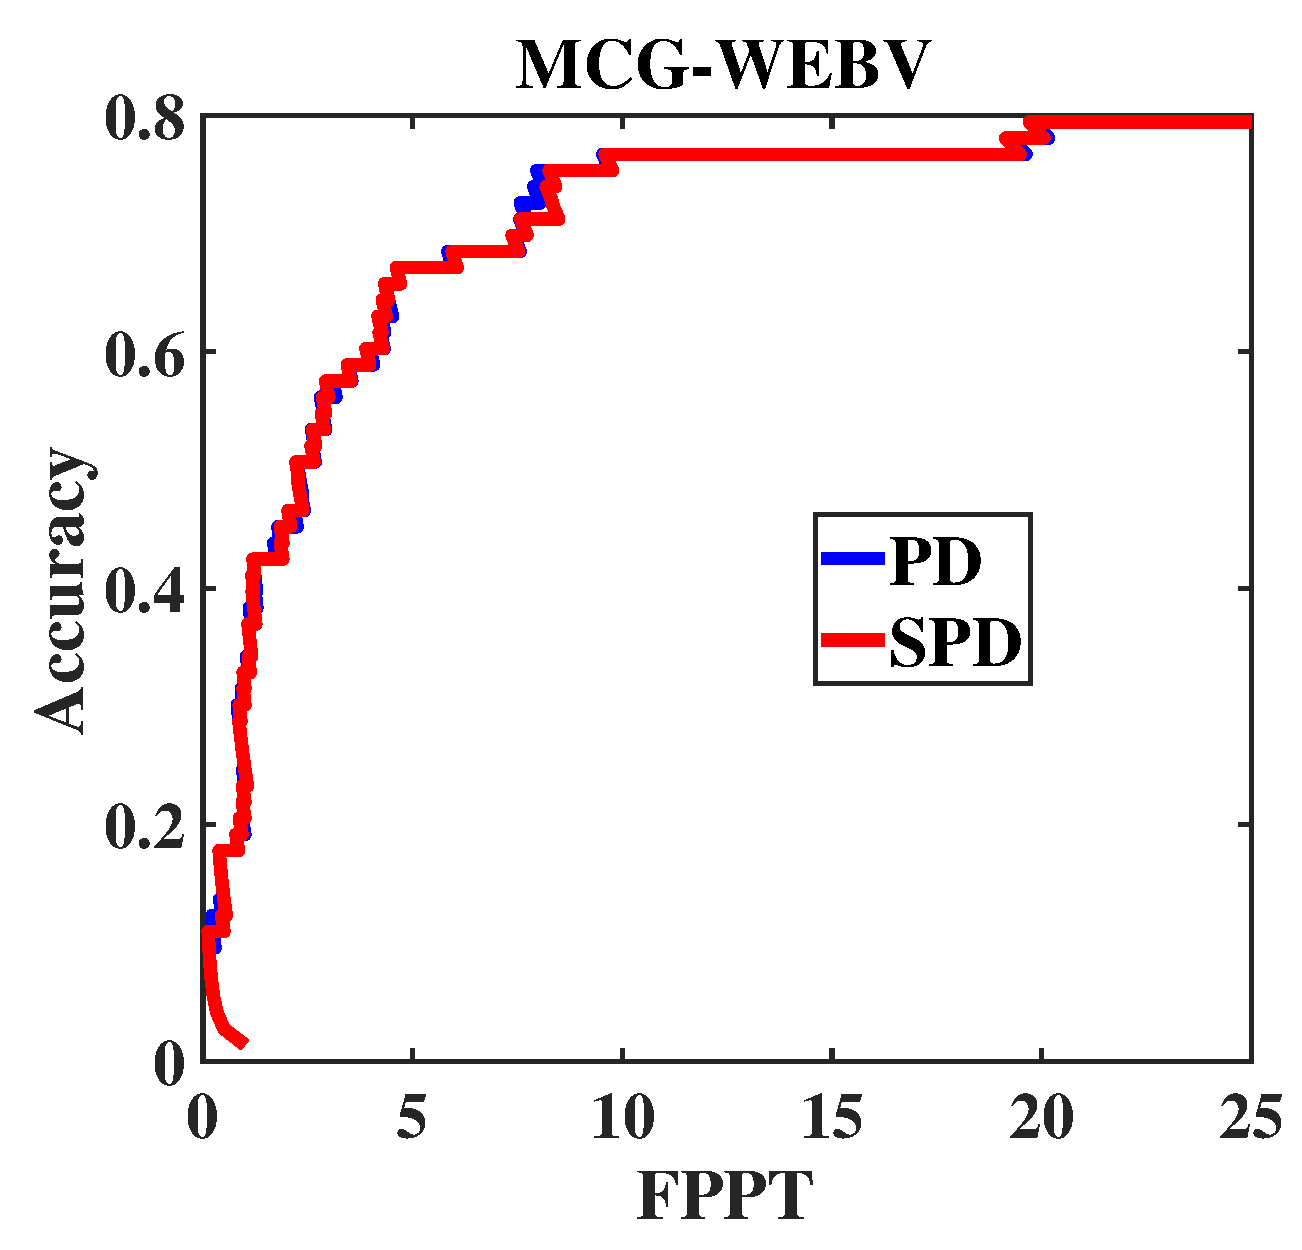
\includegraphics[width=0.31\textwidth,height=.28\textwidth]{./results/cmp-accuracy-mcg/Accuracy.eps}
\label{fig:accuracycmponmcg}
}
\subfigure[Avg-Top10F1 v.s. NDT]
{
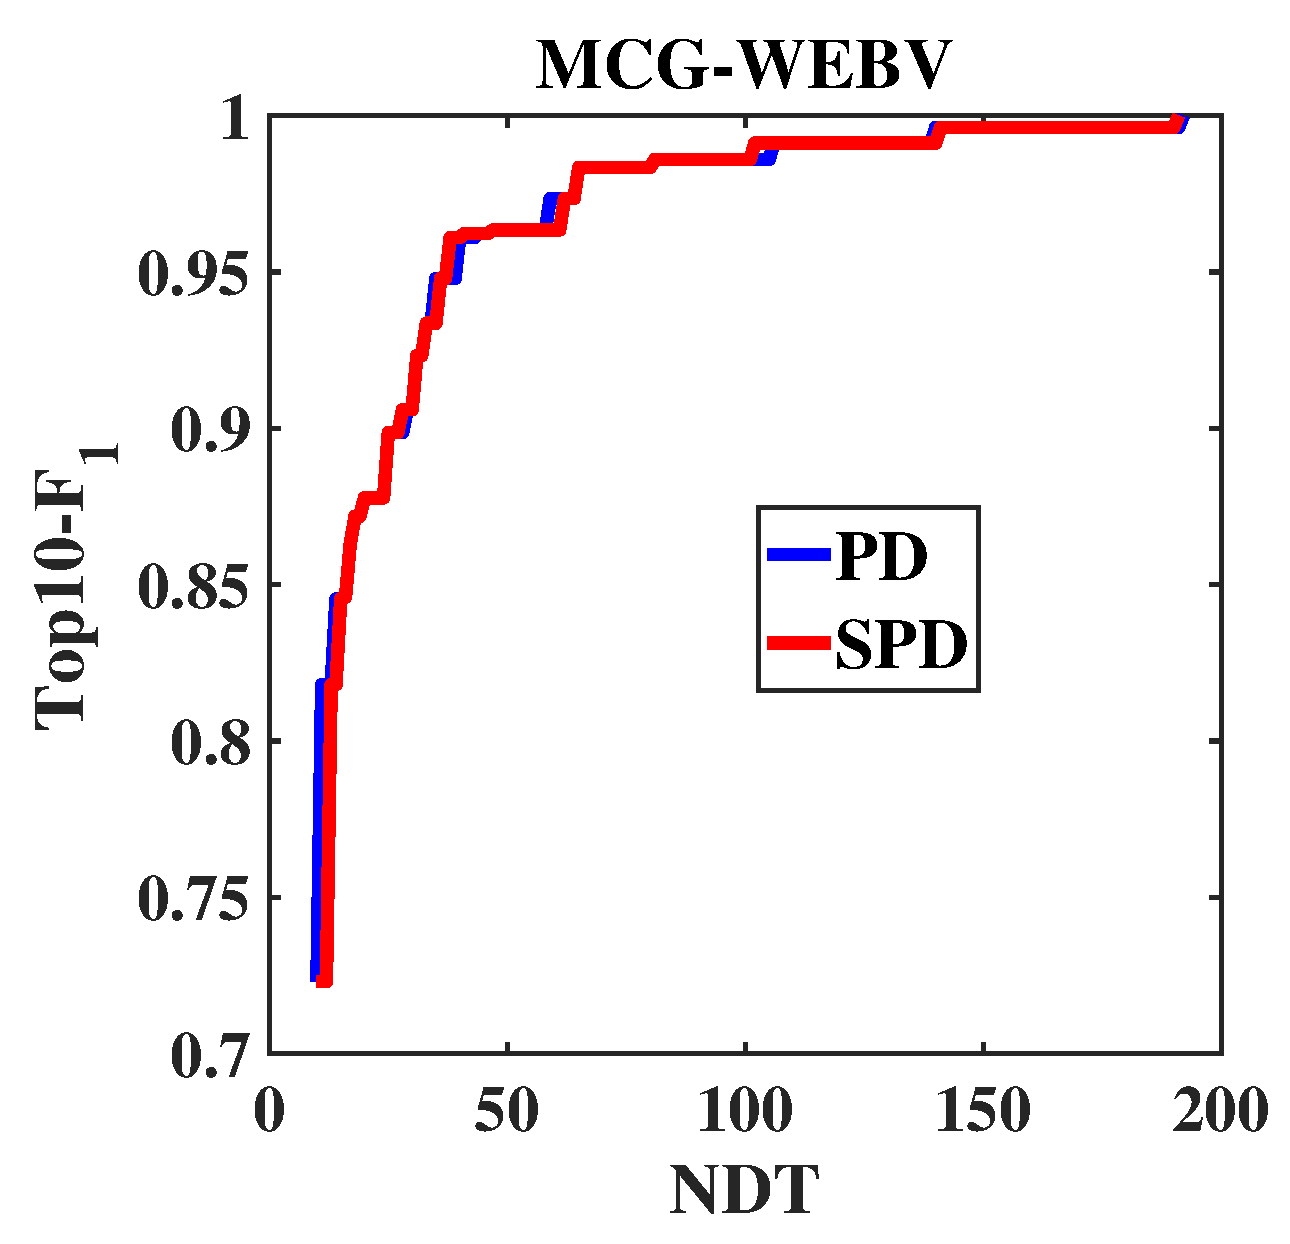
\includegraphics[width=0.31\textwidth,height=.28\textwidth]{./results/cmp-top10-mcg/Top10.eps}
\label{fig:top10cmponmcg}
}
\end{minipage}
\begin{minipage}{\textwidth}
\centering
\subfigure[Objective v.s. Time]
{
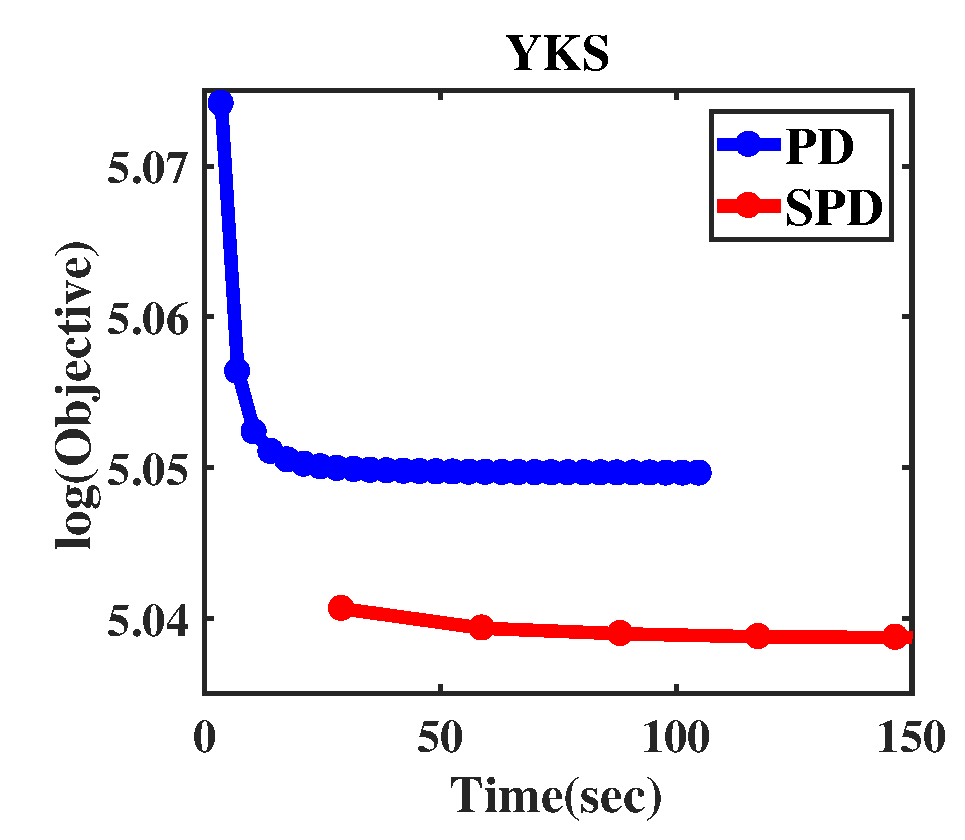
\includegraphics[width=.31\textwidth,height=.28\textwidth]{./results/cmp-objective-yks/Objective.eps}
\label{fig:objectivecmponyks}
}
\subfigure[Accuracy v.s. FPPT]
{
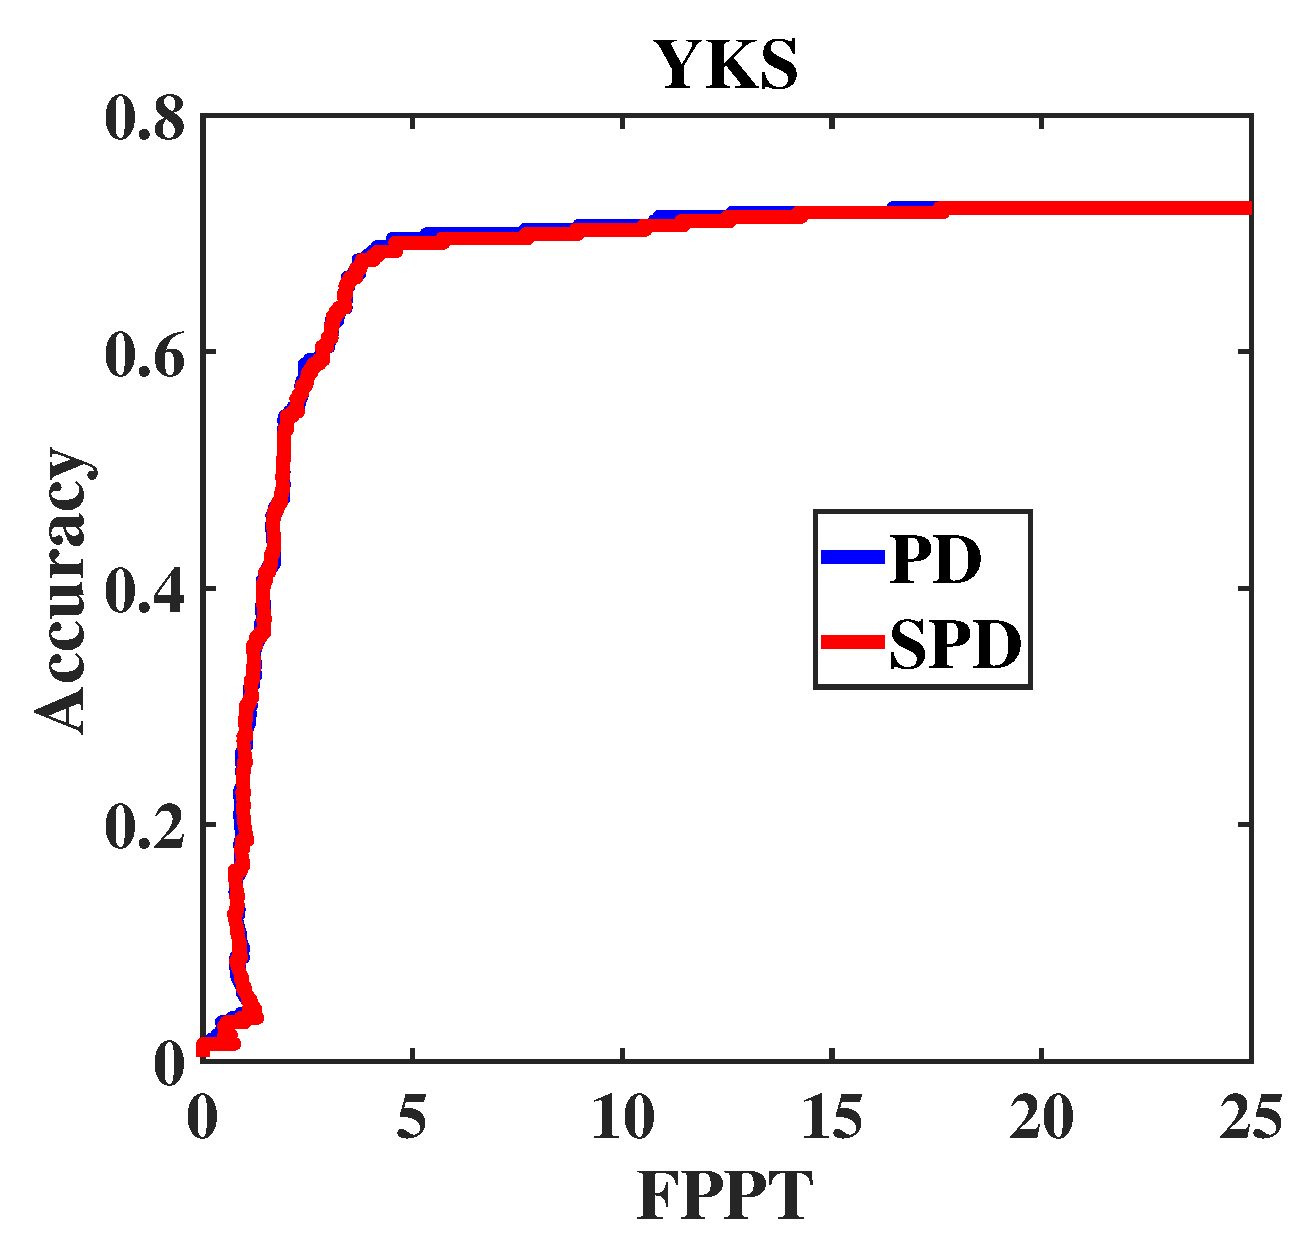
\includegraphics[width=.31\textwidth,height=.28\textwidth]{./results/cmp-accuracy-yks/Accuracy.eps}
\label{fig:accuracycmponyks}
}
\subfigure[Avg-Top10F1 v.s. NDT]
{
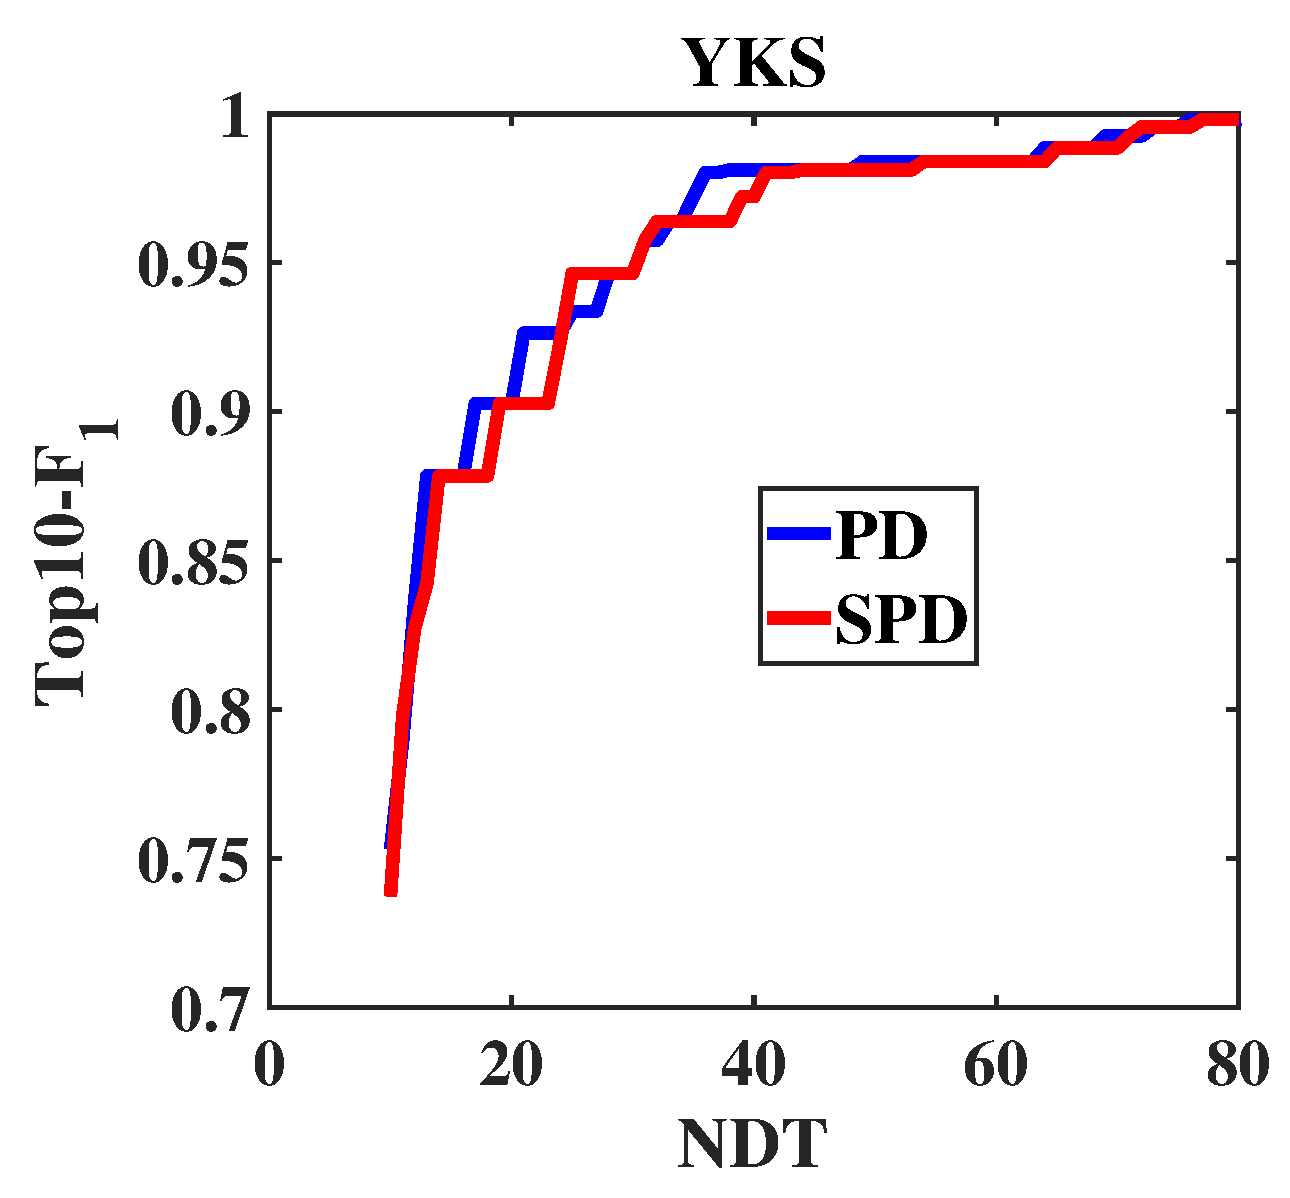
\includegraphics[width=.31\textwidth,height=.28\textwidth]{./results/cmp-top10-yks/Top10.eps}
\label{fig:top10cmponyks}
}
\end{minipage}
\caption{Comparisons between PD and SPD on MCG-WEBV and YKS.}
\label{fig:cmp-three-metric-mcg-yks}
\end{figure}

\subsection{Evaluation on Toy Dataset}
To evaluate the efficientness of SPD, we construct a large-scale toy data set by duplicating MCG-WEBV 50 times. The resulting toy data set has approximate $200,000$ webpages. In this paper, an algorithm converges to a local minimum, if the change of the log likelihood between two consecutive iterations is less than $10^{-5}$. The speedup is a ratio of CPU time taken to converge to a local minimum between two algorithms.

Fig.~\ref{fig:toydatacmp} shows that SPD significantly outperforms PD in terms of the convergence speed. In our evaluation, SPD achieves about 12.6$\times$ speedup. Moreover, at each iteration, although the decrease of the objective function of PD is larger than that of our method, our stochastic approach costs a fewer training time than that of the batch approach. This is because that PD uses all data to perform an accurate update while SPD only uses a small fraction of data to perform an approximate update at each iteration. When training a large-scale toy dataset, PD will cost more time than SPD with one epoch of data due to the problems of computational efficiency and memory limitations. Therefore, SPD converges much faster than PD in large-scale data sets. It validates the advantage of the loss~\eqref{eqt:exponentiallyweightedmovingaverage}: one should not spend too much effort on accurately minimizing the empirical loss. In addition, just like gradient descent, PD suffers from local minima issue while SPD can avoid it, which make SPD can converge to a smaller value than PD.



\subsection{Comparisons With State-Of-The-Art Algorithms}
Fig.~\ref{fig:cmp-three-metric-mcg-yks} shows the comparisons between PD and SPD on both MCG-WEBV and YKS data sets.  Figs.~\ref{fig:accuracycmponmcg}, \ref{fig:accuracycmponyks}, \ref{fig:top10cmponmcg}, and \ref{fig:top10cmponyks} illustrate that SPD achieves the similar performances to that of PD. Figs.~\ref{fig:objectivecmponmcg} and~\ref{fig:objectivecmponyks} show that SPD can get a lower log likelihood than PD. It means that SPD can converge to a smaller value with no drop in performance. Due to these two data sets are all small, PD costs fewer time than SPD with one epoch of data. Therefore, PD converges faster than SPD in small-scale data sets.


\subsection{Parameter Analysis}

\subsubsection{The Size of Mini-Batch:}
Fig.~\ref{fig:minibatch-cmp-three-metric-mcg} shows the effectiveness of different mini-batch size in SPD on MCG-WEBV. As shown in Fig.~\ref{fig:minibatch-cmp-three-metric-mcg}, objective values of different settings all converge to a local minimum; besides, the smaller the mini-batch is, the lower the log likelihood is. One possible reason is that a smaller mini-batch will bring a larger randomness, which may make SPD escape worse local minima and arrive at a relatively reasonable local minimum. Interestingly, the different sizes of mini-batch obtain very similar results in terms of accuracy v.s. FPPT and top-10 F$_1$ v.s. NDT. Therefor, the size of the mini-batch does not affect the effectiveness of SPD.

\begin{figure}[t!]
\centering
\begin{minipage}{\textwidth}
\subfigure[Objective v.s. Time]
{
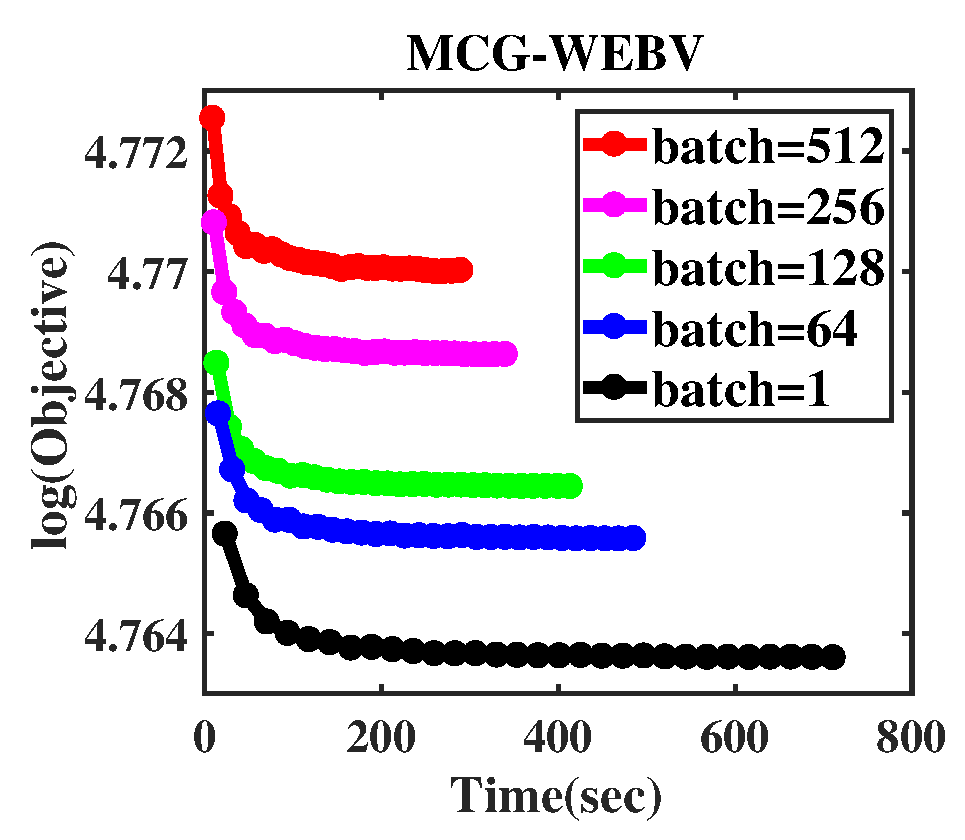
\includegraphics[width=.31\textwidth,height=.28\textwidth]{./results/minibatch-objective-mcg/Objective_time.eps}
\label{fig:minibatch-objective-mcg}
}
\subfigure[Accuracy v.s. FPPT]
{
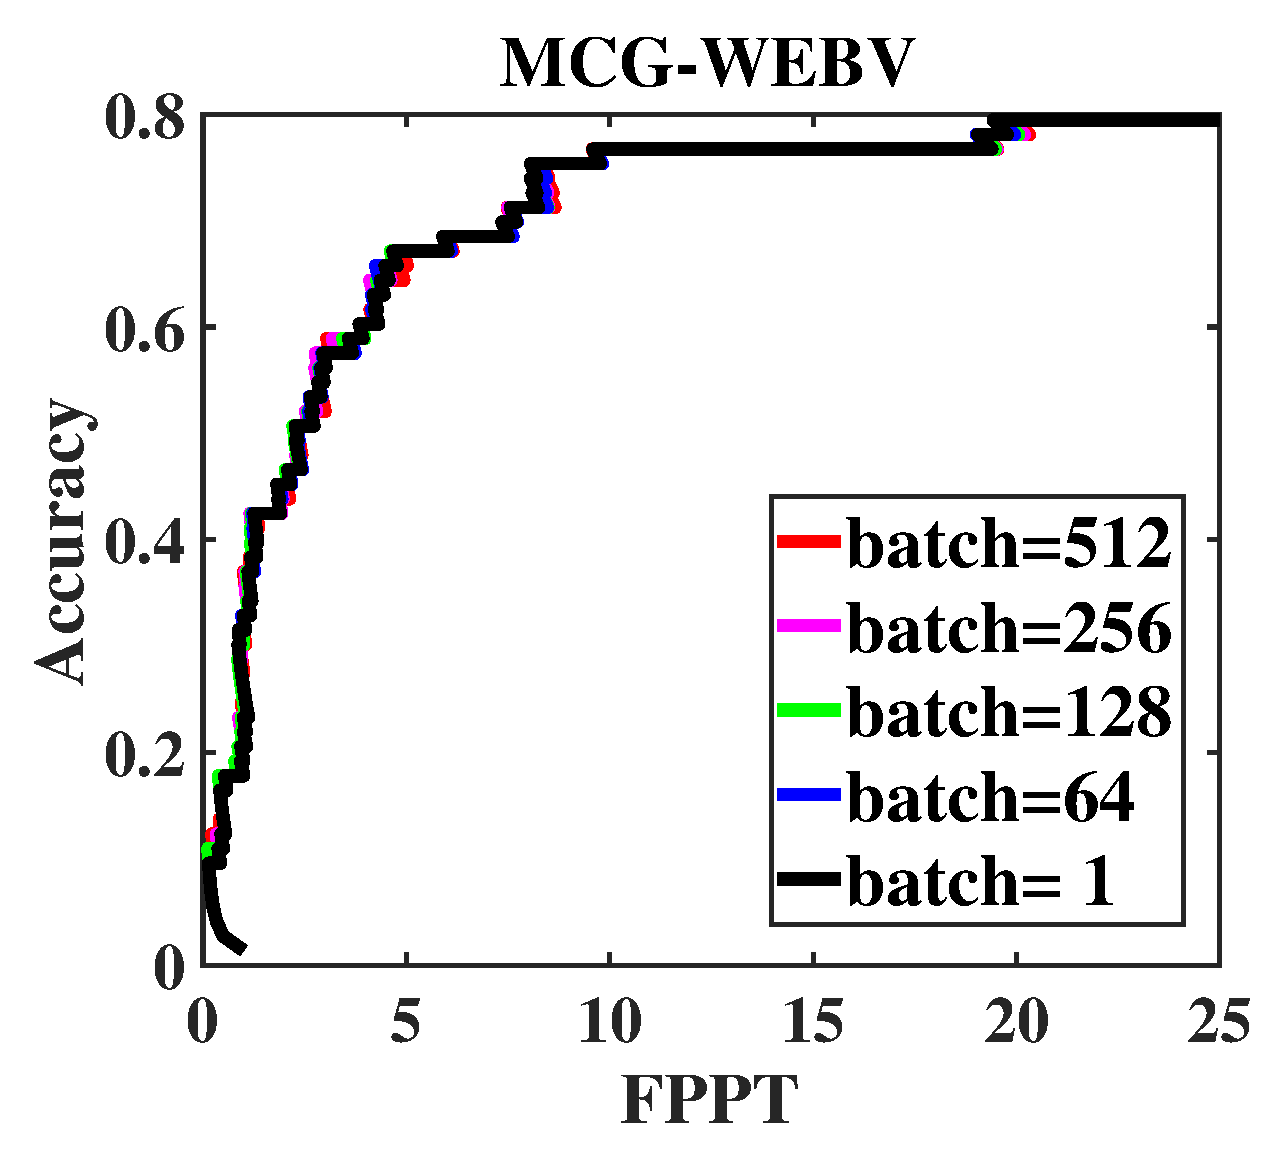
\includegraphics[width=.31\textwidth,height=.28\textwidth]{./results/minibatch-accuracy-mcg/Accuracy.eps}
\label{fig:minibatch-accuracy-mcg}
}
\subfigure[Avg-Top10F1 v.s. NDT]
{
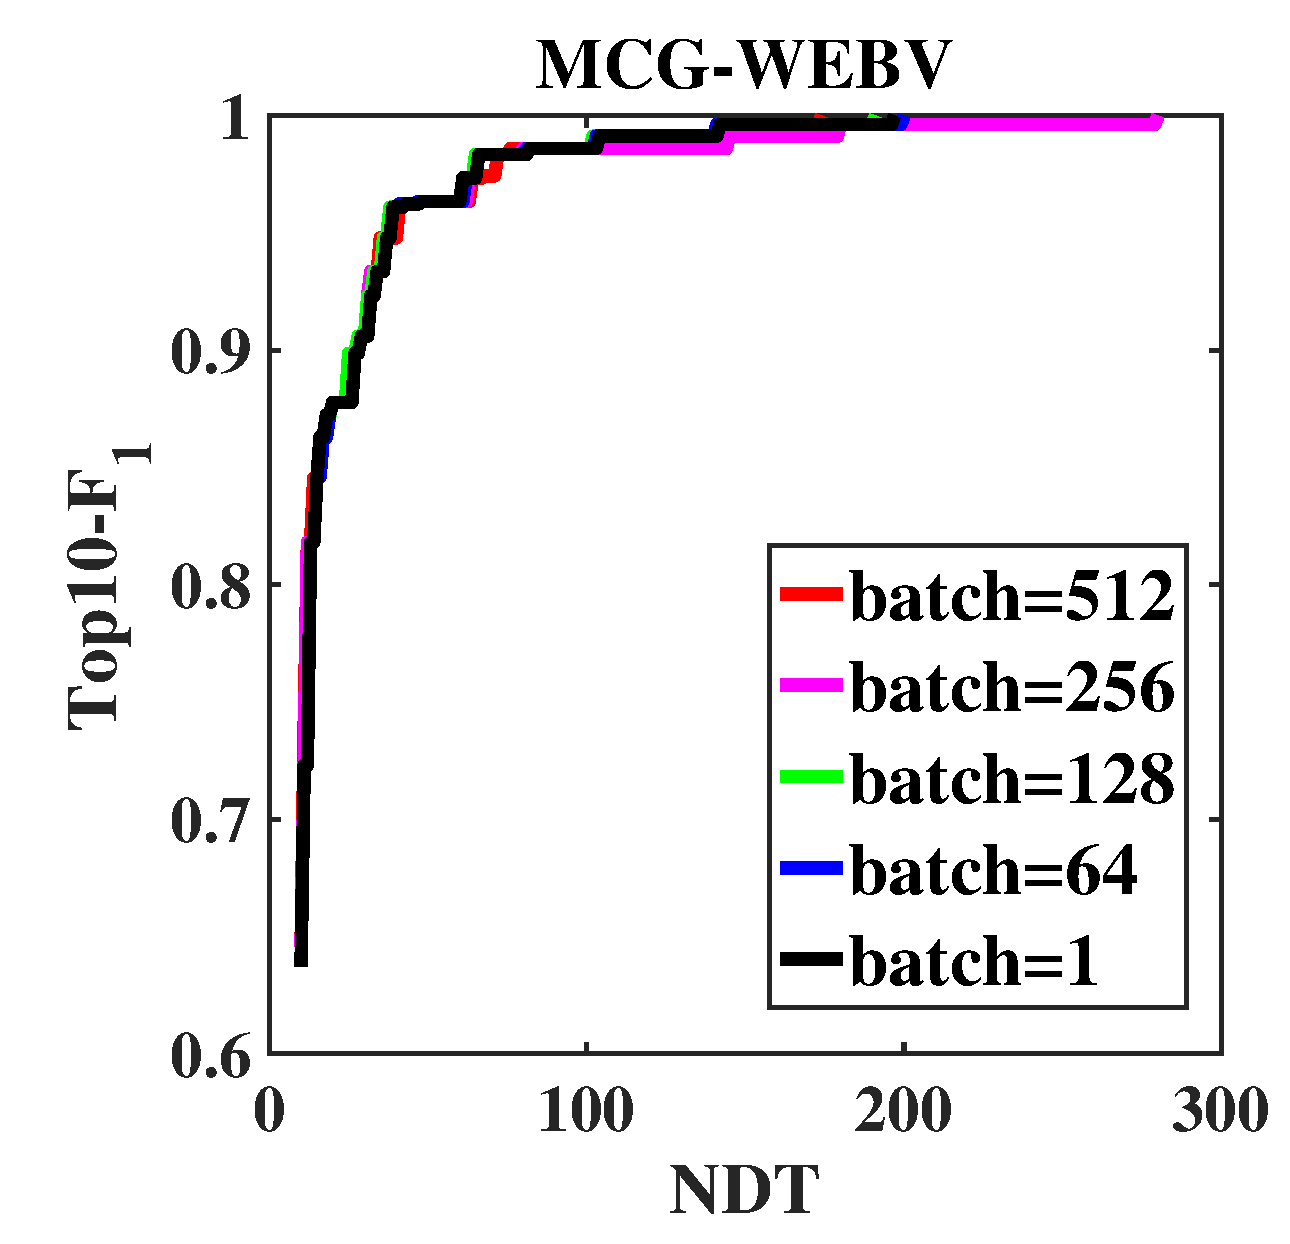
\includegraphics[width=.31\textwidth,height=.28\textwidth]{./results/minibatch-top10-mcg/Top10.eps}
\label{fig:minibatch-top10-mcg}
}
\caption{Comparisions between different batch size on MCG-WEBV.}
\label{fig:minibatch-cmp-three-metric-mcg}
\end{minipage}
\end{figure}

\subsubsection{Weight Parameters  $\alpha$ and $\beta$:}

\begin{figure}[ht!]
\centering
\begin{minipage}{1.0\textwidth}
\subfigure[Objective v.s. Time]
{
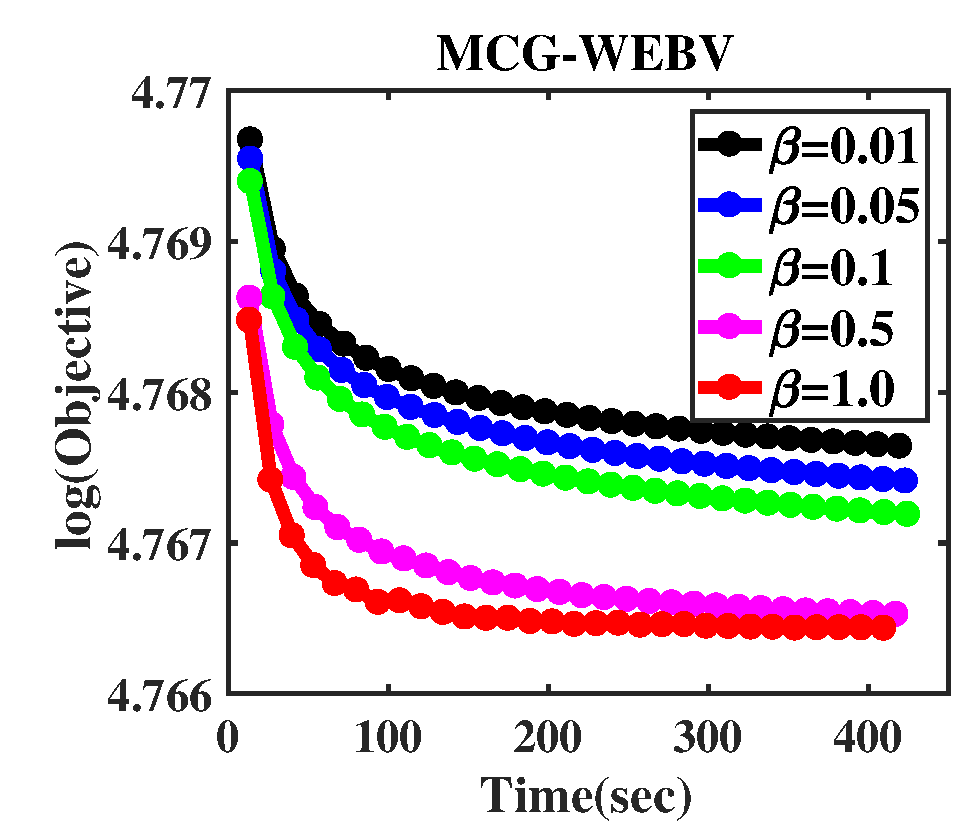
\includegraphics[width=.31\textwidth,height=.28\textwidth]{./results/beta-objective-mcg/Objective_time_Beta.eps}
\label{fig:objectivebeta}
}
\subfigure[Accuracy v.s. FPPT]
{
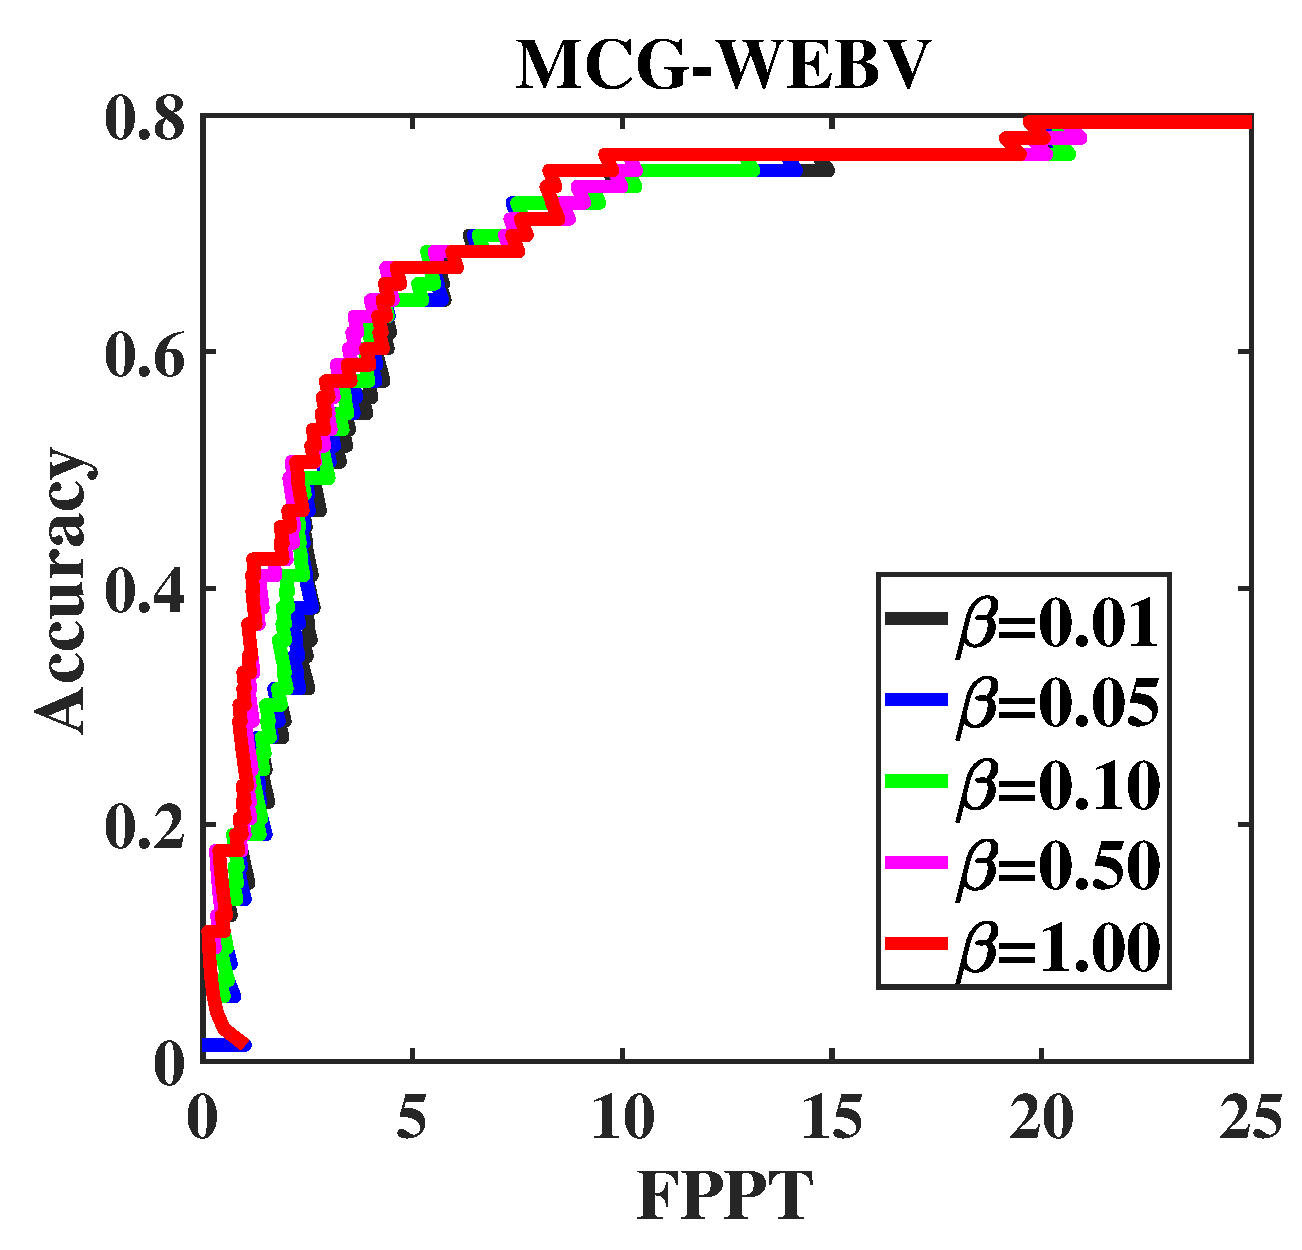
\includegraphics[width=.31\textwidth,height=.28\textwidth]{./results/beta-accuracy-mcg/Accuracy_Beta.eps}
\label{fig:accuracybeta}
}
\subfigure[Avg-Top10F1 v.s. NDT]
{
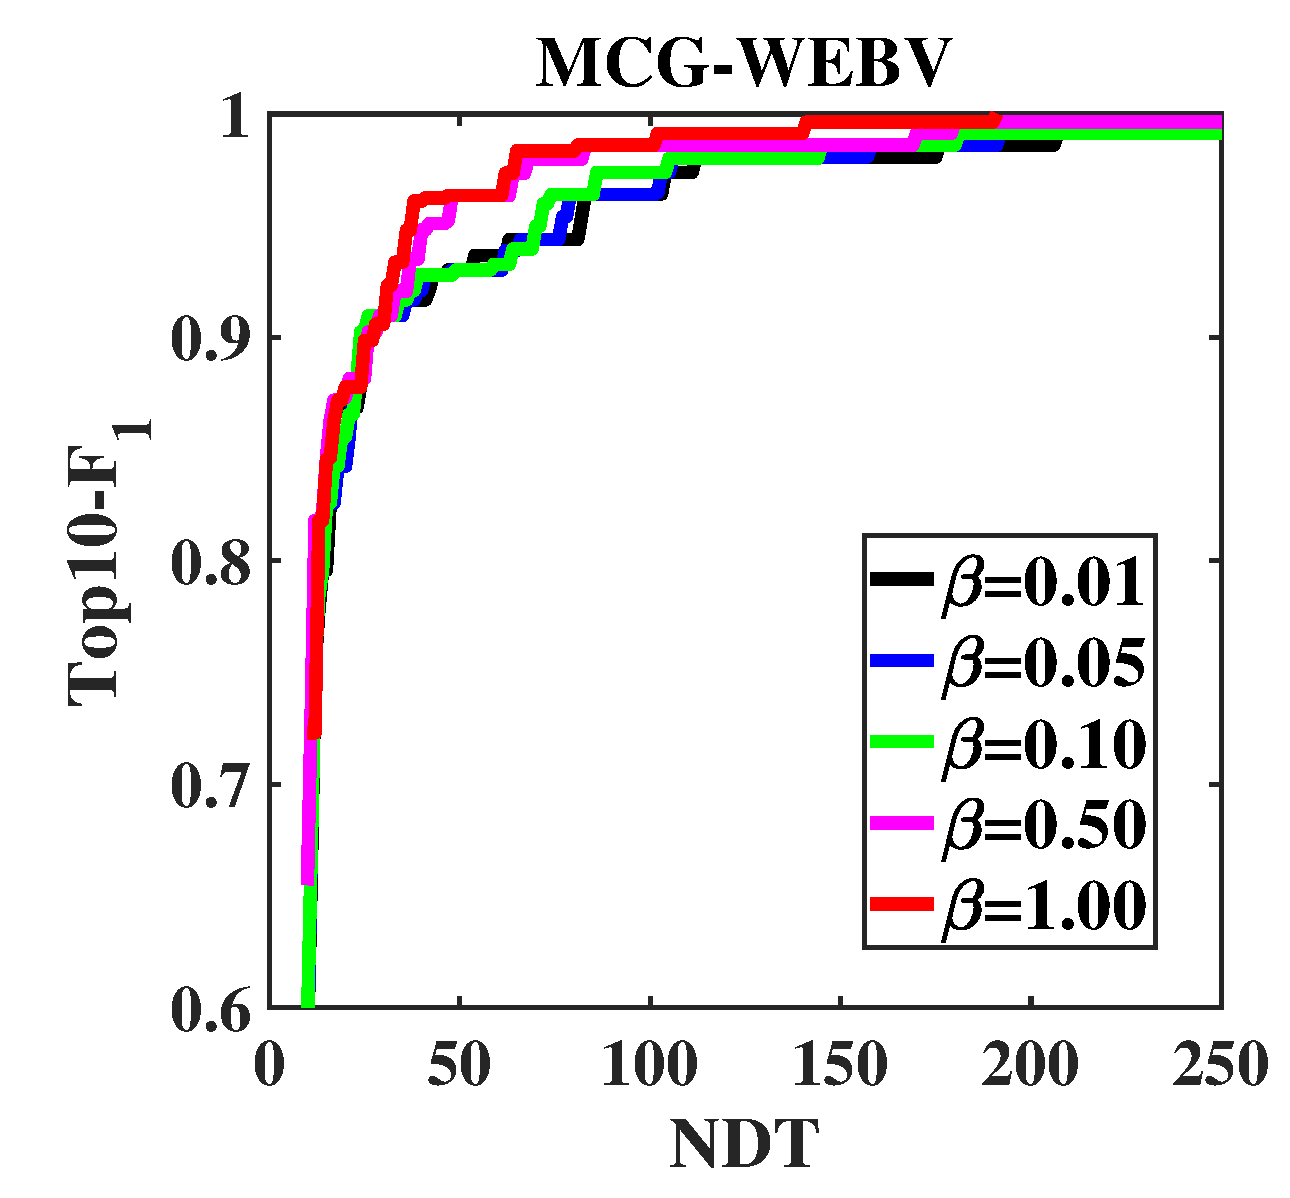
\includegraphics[width=.31\textwidth,height=.28\textwidth]{./results/beta-top10-mcg/Top10_Beta.eps}
\label{fig:top10beta}
}
\caption{Comparisons among different $\beta$ in SPD on MCG-WEBV.}
\label{fig:differentbeta}
\end{minipage}
\end{figure}

In our implementation, we use a decreasing weight in~\eqref{eqt:weightupdate}, where $\beta$ is a initial weight, and $\alpha$ is a decay factor. Fig.~\ref{fig:differentbeta} shows comparisons among various $\beta$ when other parameters are fixed, \emph{i.e.}, $\alpha$=$0$, mini-batch=$128$, and $epoch=30$. Fig.~\ref{fig:objectivebeta} illustrates the effectiveness of $\beta$ on the convergence rate. As expected, the larger $\beta$ is, the faster the convergence speed of SPD is. Because a larger $\beta$ will make the surrogate function quickly adapt to the latest surrogate one. From Fig.~\ref{fig:accuracybeta} and Fig.~\ref{fig:top10beta}, we find that a larger $\beta$ not only results in a faster convergence speed, but also obtains a better performance.



\begin{figure}[t!]
\centering
\begin{minipage}{1.0\textwidth}
\subfigure[Objective v.s. Time]
{
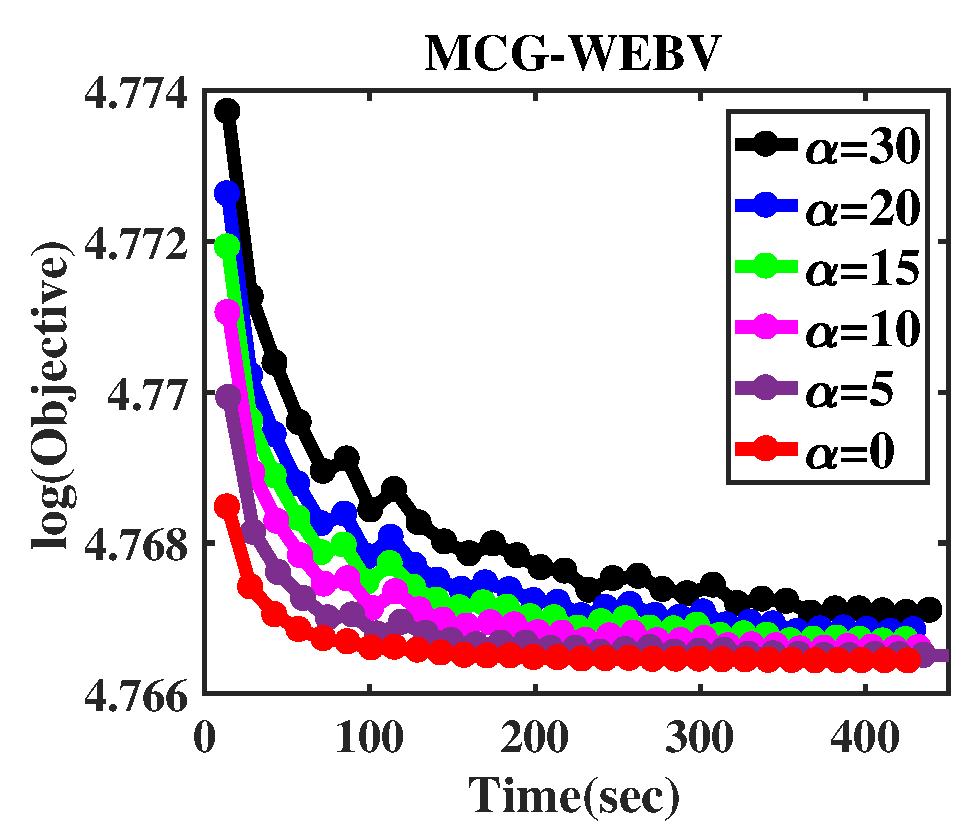
\includegraphics[width=.31\textwidth,height=.28\textwidth]{./results/alpha-objective-mcg/Objective_time_Alpha.eps}
\label{fig:objectivealpha}
}
\subfigure[Accuracy v.s. FPPT]
{
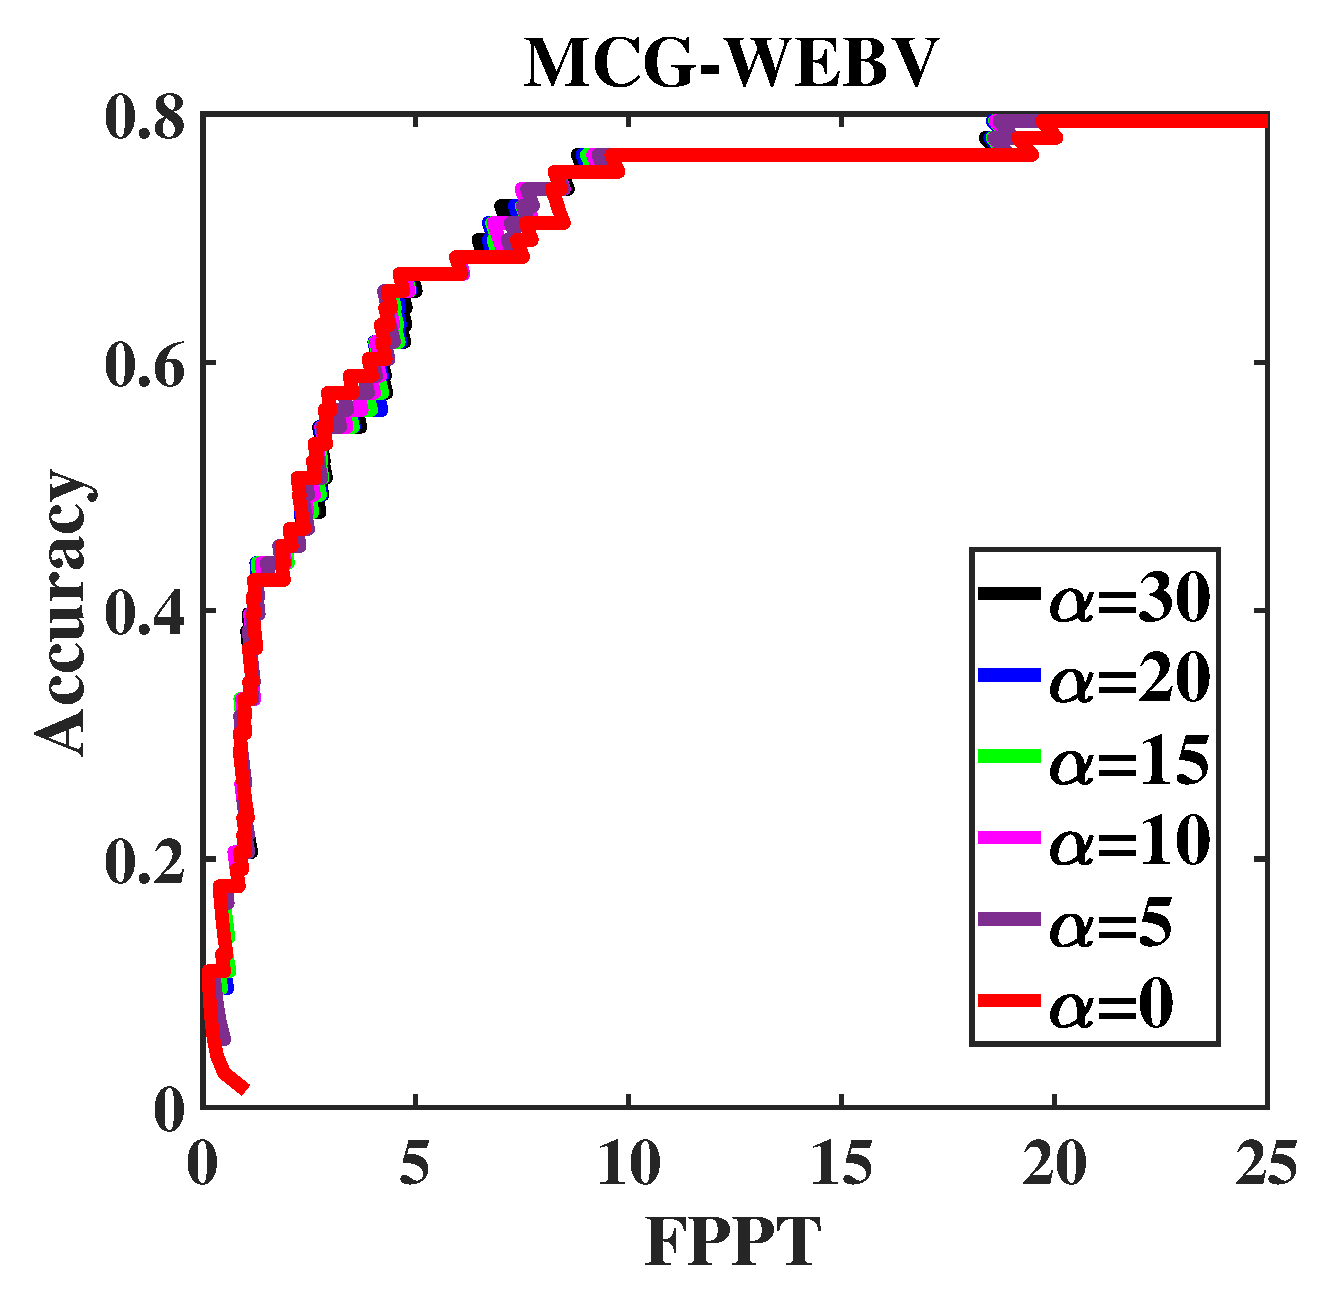
\includegraphics[width=.31\textwidth,height=.28\textwidth]{./results/alpha-accuracy-mcg/Accuracy_Alpha.eps}
\label{fig:accuracyalpha}
}
\subfigure[Avg-Top10F1 v.s. NDT]
{
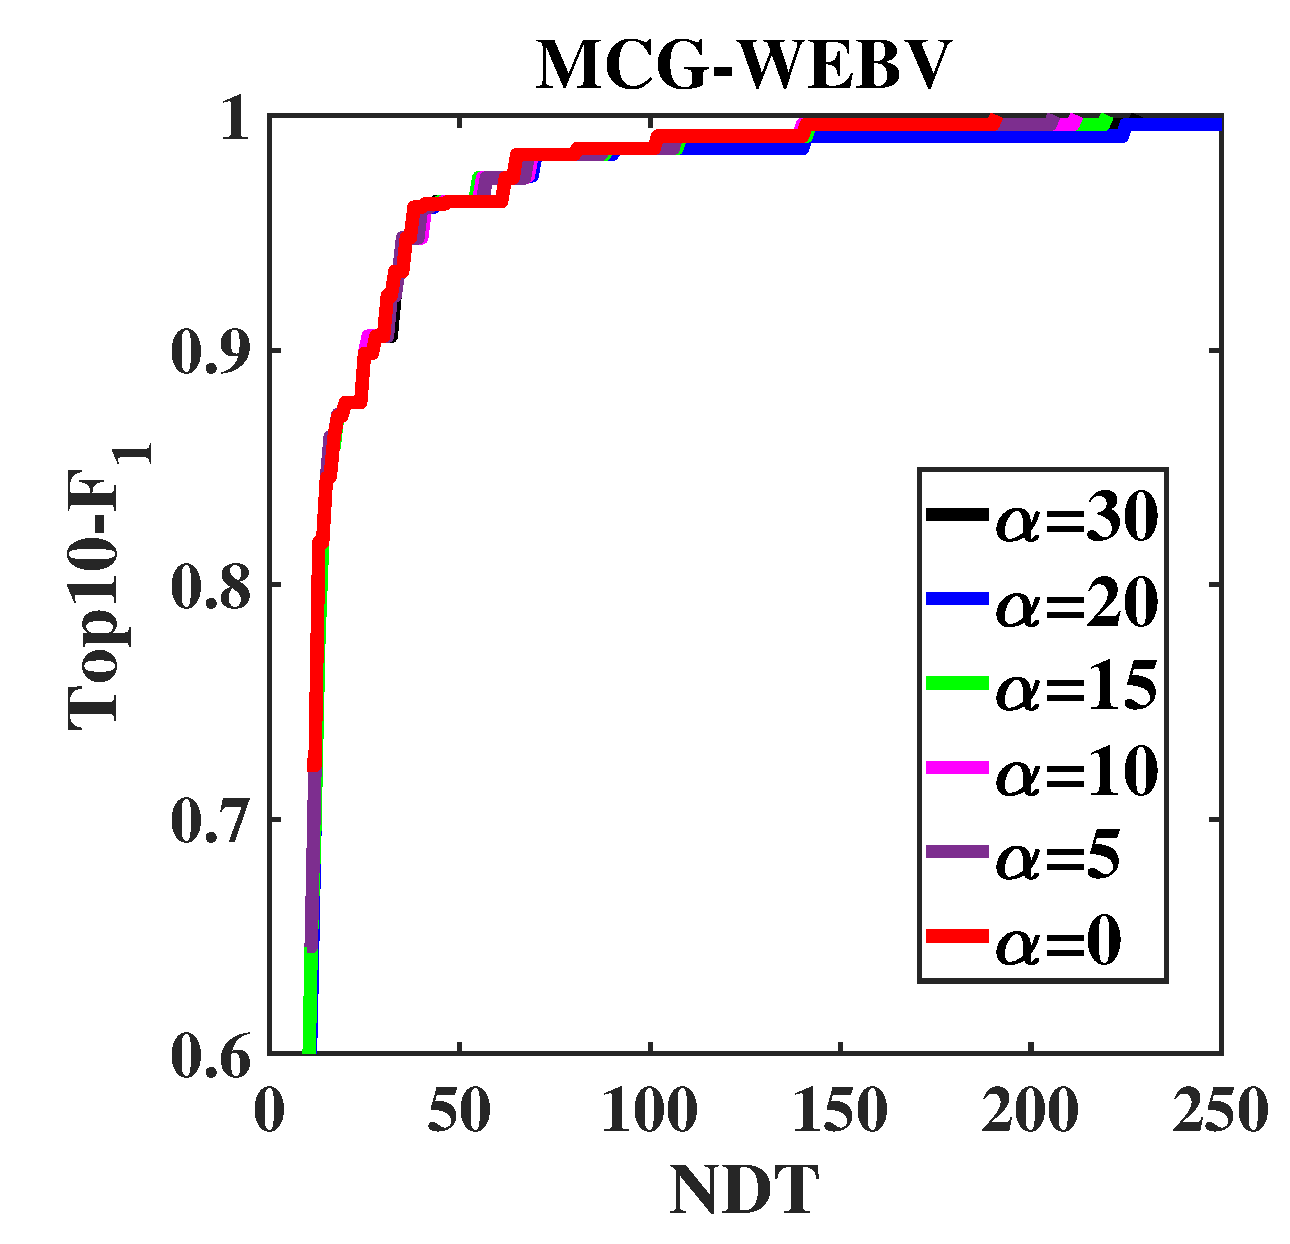
\includegraphics[width=.31\textwidth,height=.28\textwidth]{./results/alpha-top10-mcg/Top10_Alpha.eps}
\label{fig:top10alpha}
}
\caption{Comparison among different $\alpha$ in SPD on MCG-WEBV.}
\label{fig:differentalpha}
\end{minipage}
\end{figure}

Fig.~\ref{fig:differentalpha} shows comparisons among various $\alpha$ when the other parameters are fixed, \emph{i.e.}, $\beta$=$1$, mini-batch=$128$, $epoch=30$. Fig.~\ref{fig:objectivealpha} shows that a smaller $\alpha$ leads to a smoother objective function curves. Because a smaller $\alpha$ not only makes $\beta$ decay faster, but also makes SPD stable to the latest surrogates. These different settings of $\alpha$ converges to a local minimum.

In summary, although different settings of $\alpha$ and $\beta$ influence the convergence speed of SPD, both accuracy v.s. FPPT and top-10 $F_1$ v.s. NDT are robust to these parameters.

\section{Conclusion}
\label{sec:conclusion}
In this paper, we have introduced a SPD approach Sthat gracefully scales to large-scale data set for web topic detection. We have shown that our algorithm is comparable to the state-of-the-art algorithms in terms of accuracy for web topic detection. Moreover, a large-scale data set is also synthesized artificially to confirm the advantage of convergence speed. In the future, we would incorporate asynchronous parallel strategy into SPD due to the multicore systems; besides, incorporating online learning is another interesting direction.
\\
\\
\textbf{Acknowledgements.} This work was supported in part by National Natural Science Foundation of China: 61332016, 61472389, 61672069, 61872333, 61650202 and U1636214, in part by Key Research Program of Frontier Sciences, CAS: QYZDJ-SSW-SYS013.


% ---- Bibliography ----
%
% BibTeX users should specify bibliography style 'splncs04'.
% References will then be sorted and formatted in the correct style.

\bibliographystyle{splncs04}
\bibliography{MMM_SPD_Camera-ready}

\end{document}
